\documentclass{standalone}
\usepackage{tikz}
\usetikzlibrary{patterns}
\usetikzlibrary{positioning}
\usetikzlibrary{patterns, positioning}
\usetikzlibrary{shapes.misc}
\usepackage[outline]{contour}
\contourlength{1.5pt} 
\usepackage[sfdefault]{ClearSans}

\begin{document}
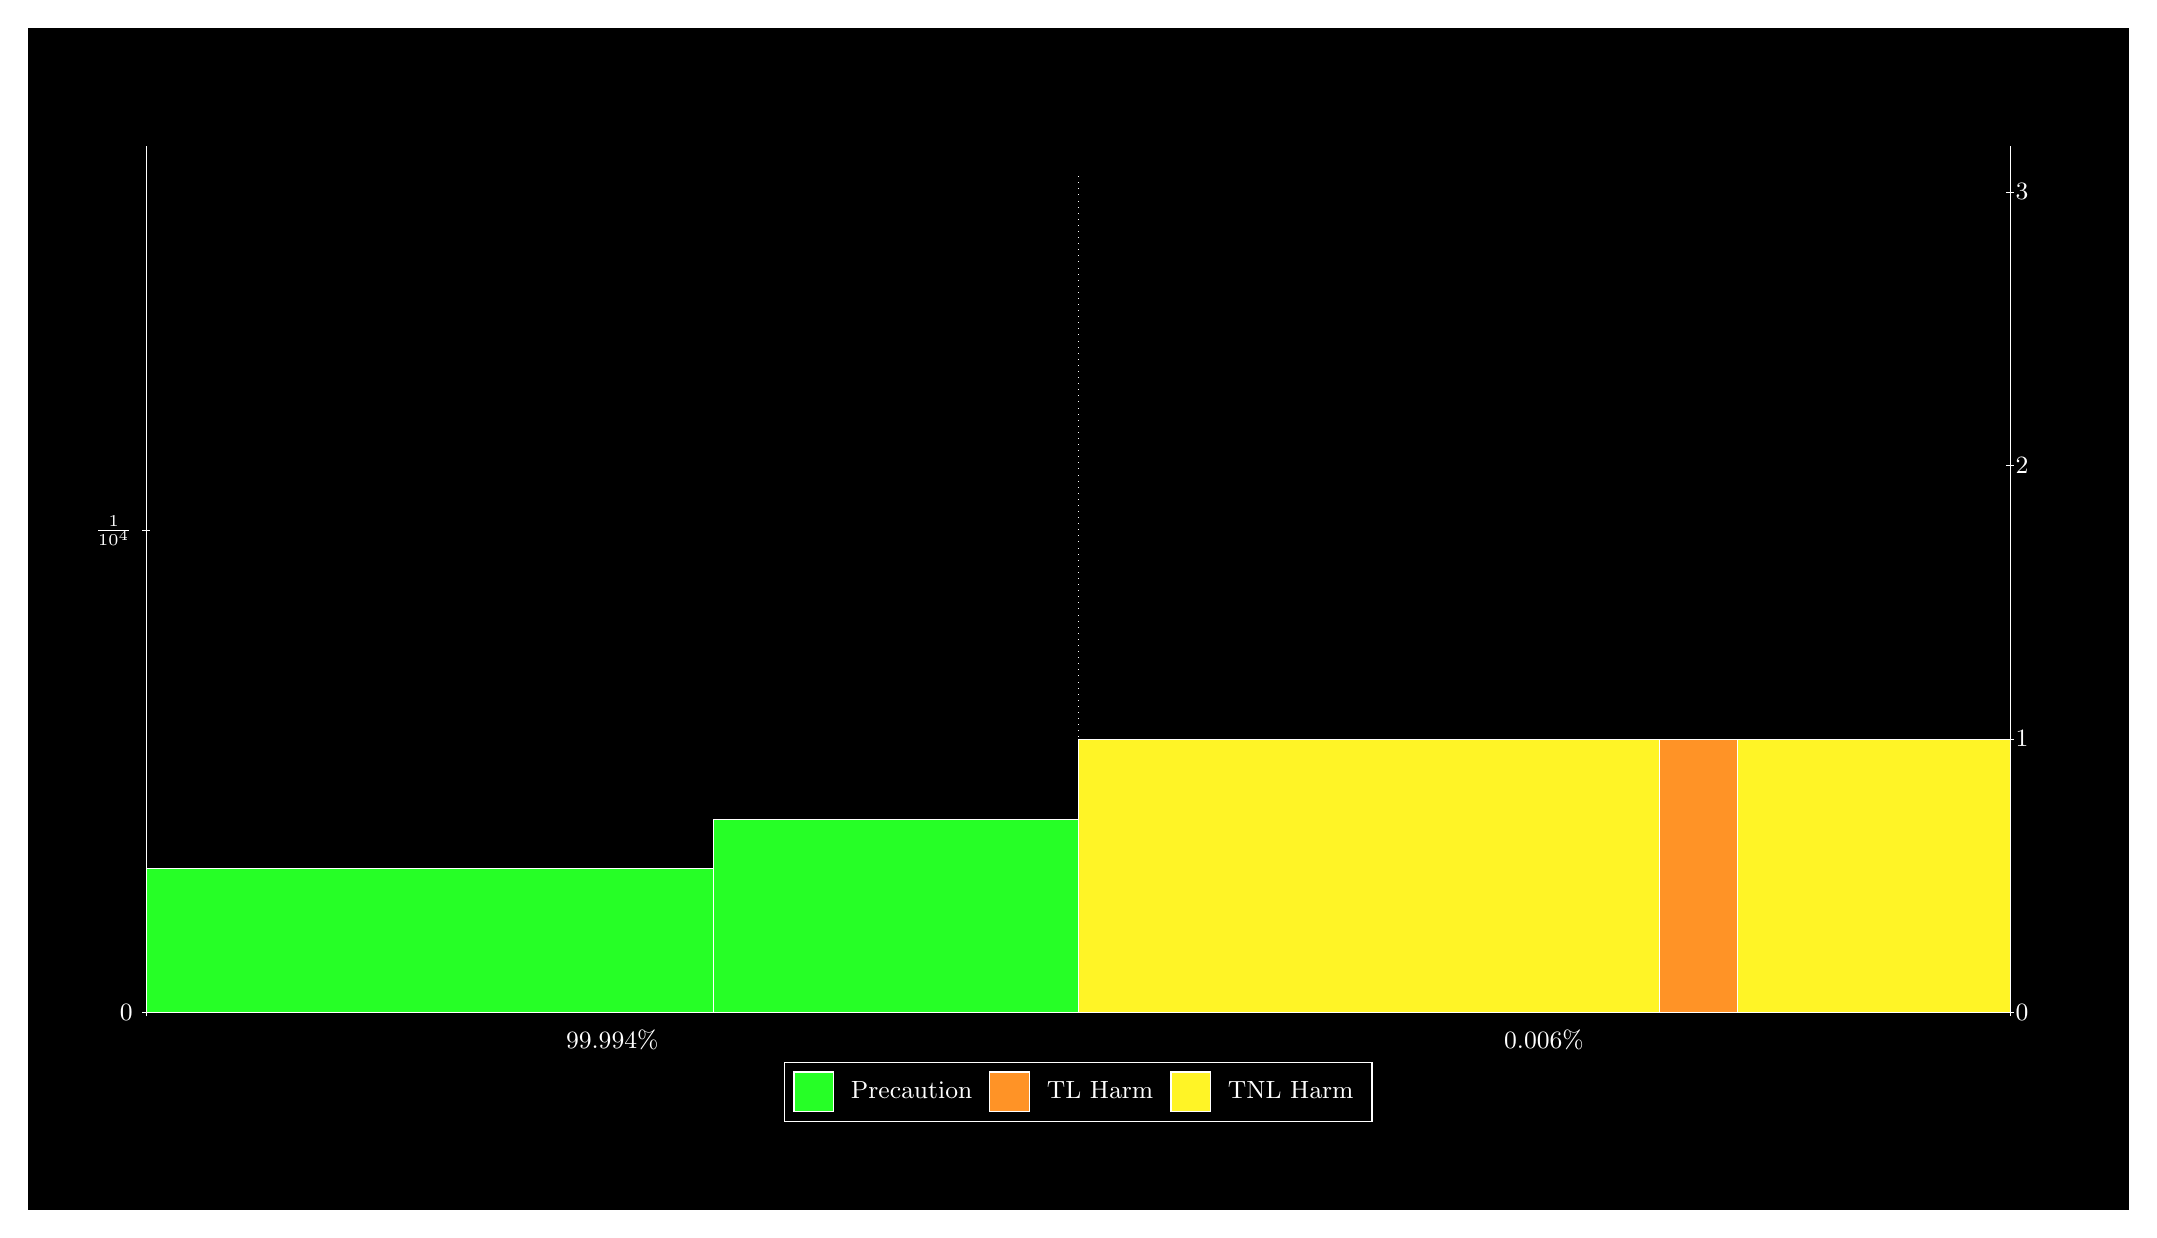
\begin{tikzpicture}
\draw[fill=black] (0,0) rectangle (26.667,15);
\draw[fill=green!85,draw=white,very thin] (1.5,2.5) rectangle (8.696,4.3364);
\draw[fill=green!85,draw=white,very thin] (8.696,2.5) rectangle (13.333,4.9486);
\draw[fill=green!85,draw=white,very thin] (13.333,2.5) rectangle (20.715,2.5001);
\draw[fill=yellow!85,draw=white,very thin] (13.333,2.5001) rectangle (20.715,5.9736);
\draw[fill=green!85,draw=white,very thin] (20.715,2.5) rectangle (21.71,2.5001);
\draw[fill=orange!85,draw=white,very thin] (20.715,2.5001) rectangle (21.71,5.9736);
\draw[fill=green!85,draw=white,very thin] (21.71,2.5) rectangle (25.167,2.5001);
\draw[fill=yellow!85,draw=white,very thin] (21.71,2.5001) rectangle (25.167,5.9737);
\draw[white,very thin] (1.5,2.5) -- (1.5,13.5);
\draw[white,very thin] (1.45,2.5) -- (1.55,2.5);
\node[font=\small,text=white, anchor=east] at (1.45, 2.5) {0};
\draw[white,very thin] (1.45,8.6215) -- (1.55,8.6215);
\node[font=\small,text=white, anchor=east] at (1.45, 8.6215) {$\frac{1}{10^{4}}$};

\draw[white,dotted,very thin] (13.333,2.83) -- (13.333,13.17);
\draw[white,very thin] (25.167,2.5) -- (25.167,13.5);
\draw[white,very thin] (25.117,2.5) -- (25.217,2.5);
\node[font=\small,text=white, anchor=west] at (25.117, 2.5) {0};
\draw[white,very thin] (25.117,5.9735) -- (25.217,5.9735);
\node[font=\small,text=white, anchor=west] at (25.117, 5.9735) {1};
\draw[white,very thin] (25.117,9.4471) -- (25.217,9.4471);
\node[font=\small,text=white, anchor=west] at (25.117, 9.4471) {2};
\draw[white,very thin] (25.117,12.921) -- (25.217,12.921);
\node[font=\small,text=white, anchor=west] at (25.117, 12.921) {3};

\draw[white,very thin] (1.5,2.5) -- (25.167,2.5);
\draw[white,very thin] (1.5,2.45) -- (1.5,2.55);
\node[font=\small,text=white, anchor=north] at (1.5, 2.45) {};
\draw[white,very thin] (25.167,2.45) -- (25.167,2.55);
\node[font=\small,text=white, anchor=north] at (25.167, 2.45) {};

\node[font=\small,text=white,anchor=south] at (7.4167, 1.9) {99.994\%};
\node[font=\small,text=white,anchor=south] at (19.25, 1.9) {0.006\%};
\draw (13.3333,2.5) node (B) {};
\begin{scope}[align=center]
\matrix[scale=0.5,draw=white,below=0.5cm of B,nodes={draw},column sep=0.1cm]{
\node[rectangle,draw,minimum width=0.5cm,minimum height=0.5cm,fill=green!85]{}; & \node[draw=none,font=\small,text=white]{Precaution}; &
\node[rectangle,draw,minimum width=0.5cm,minimum height=0.5cm,fill=orange!85]{}; & \node[draw=none,font=\small,text=white]{TL Harm}; &
\node[rectangle,draw,minimum width=0.5cm,minimum height=0.5cm,fill=yellow!85]{}; & \node[draw=none,font=\small,text=white]{TNL Harm}; \\\\
};\end{scope}

\end{tikzpicture}
\end{document}